\chapter{Work Done}

\section{Compiler Infrastructures}
There are various compiler infrastructures available as options for experimental compiler research. We looked into some of the most popular ones: SUIF, GCC and LLVM.

\textbf{SUIF Compiler System}\cite{suif} is a compiler infrastructure made freely available by the Stanford SUIF Compiler Group to support research in optimizing and parallelizing compilers and uses a program representation, also called SUIF (Stanford University Intermediate Format). It supports C, C++, Fortran and Java as frontends and C, x86, Alpha and MachSUIF as backends. It provides an extensible SUIF representation which allows programmers to extend the representation without requiring updating the infrastruture.

\textbf{GCC (GNU Compiler Collection)}\cite{gcc} is a compiler system produced by the GNU Project which supports various programming languages. GCC is adopted as the standard compiler by most of the modern UNIX-like operating systems, including Linux and BSD. Frontends are available for C, C++, Objective-C, Objective-C++, Fortran, Java, Ada, and Go. It has been ported to a wide variety of processor architecures and is also available for most embedded platforms.

\textbf{LLVM}\cite{llvm} is a fairly new compiler infrastructure developed at University of Illinois, which is designed for compile-time, link-time, run-time and idle-time optimizations of programs. It has a language-agnostic design, which allows it to support a wide variety of frontends, some of which include C, C++, Objective-C, D, Fortran and Ada among others. Clang, LLVM frontend for C-like languages, claims to be much faster and to use much less memory than GCC\cite{clang}. But LLVM supports fewer targets compared to GCC.

We choose GCC as our implementation platform as it is a popular, professional, open-source compiler and could yield more realistic results.

\section{Structure of GCC}
Like most compilers, the compilation process of a GCC-based compiler can be conceptually split up in three phases\cite{gcc-structure}:

\begin{itemize}
	\item There is a separate front end for each supported language. A front end takes the source code, translates that source code into a semantically equivalent, language independent abstract syntax tree (AST). The syntax and semantics of this AST are defined by the GIMPLE language, the highest level language independent intermediate representation GCC has.
	\item This AST is then run through a list of target independent code transformations that take care of constructing a control flow graph, and optimizing the AST for optimizing compilations, lowering to non-strict RTL (expand), and running RTL based optimizations for optimizing compilations. The non-strict RTL is handed over to more low-level passes.
	\item The low-level passes are the passes that are part of the code generation process. The first job of these passes is to turn the non-strict RTL representation into strict RTL. Other jobs of the strict RTL passes include scheduling, doing peephole optimizations, and emitting the assembly output.
\end{itemize}
	Neither the AST nor the non-strict RTL representations are completely target independent, but the GIMPLE language is target independent.
	Compiler pipeline for GCC can be seen in figure \ref{fig:pipeline}.

\begin{figure}[htb]
\centering
\includegraphics[scale=0.3]{./gcc-pipeline}
\caption{Compiler Pipeline\cite{dnovillo}}
\label{fig:pipeline}
\end{figure}


\subsection{IR Forms}
GCC internally uses several intermediate forms:
\begin{itemize}
	\item GENERIC
	\item GIMPLE
	\item Register Transfer Language (RTL)
\end{itemize}

\subsubsection{GENERIC}
GENERIC\cite{generic} is an intermediate representation language aimed to provide a language-independent way of representing an entire function in trees. The C, C++ and Java front ends of GCC produce GENERIC directly in the front end. Other front ends instead have different intermediate representations after parsing and convert these to GENERIC.
\subsubsection{GIMPLE}
GIMPLE\cite{gimple} is a three-address representation derived from GENERIC by breaking down GENERIC expressions into tuples of no more than 3 operands (with some exceptions like function calls) using temporary variables. All frontends of GCC convert their IR forms to GIMPLE (via GENERIC) for the middle stage of GCC, which does most of the code analysis and optimization.
\subsubsection{Register Transfer Language}
Register transfer language (RTL)\cite{rtl} is an intermediate representation (IR) that is very close to assembly language (low-level). In GCC, RTL is generated from the GIMPLE representation, transformed by various passes in the GCC `middle-end', and then converted to assembly language.

\subsection{GCC Plugin Mechanism}
GCC supports plugin mechanism for implementing optimization passes (manipulating GIMPLE form). The pass manager takes care of choosing and running all the available passes and their order on the program AST. A plugin could be either a static plugin or a dynamic one.

We choose to implement our pass as a dynamic plugin since it's easier to integrate it with GCC without recompiling. Figure \ref{fig:dynamic-plugin} shows how a dynamic plugin can be inserted at a desired point in the list of passes.

\begin{figure}[htb]
\centering
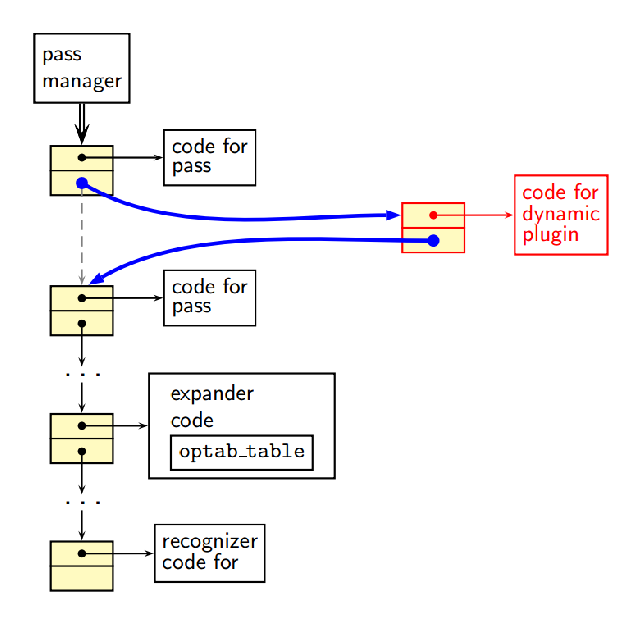
\includegraphics[scale=0.65]{./dynamic-plugin1}
\caption{Dynamic Plugin Mechanism in GCC\cite{grc}}
\label{fig:dynamic-plugin}
\end{figure}
